%! Author = vojmo
%! Date = 29.01.2022

\chapter{Analýza}

\section{Kvalitativní průzkum}

%TODO: Popsat více?
Nejprve bylo potřeba zjistit, co by potenciální uživatelé aplikace ocenili, tedy získat od nich požadavky.
Zvolil jsem kvalitativní průzkum, který se narozdíl od kvantitativního zaměřuje na malou skupinu respondentů.
Pro získání odpovědí jsem si připravil sadu otevřených otázek, kterých jsem se držel při rozhovoru. Hovory byly
uskutečněny online a každy trval mezi dvaceti minutami a jednou hodinou.

Na začátek jsem představil aplikaci a poté jsem se ptal na lehčí otázky, které odlehčili situaci. Postupně jsem se
propracoval k specifičtějším otázkám. Po několika rozhovorech se již odpovědi začaly opakovat a tak jsem už další
neprováděl.

\subsection{Seznam otázek}
\begin{itemize}
    \item Jak často vaříš?
    \item Co ti na vaření vadí a co tě naopak baví?
    \item Jaké recepty používáš?
    \item Používáš online recepty (co ti na nich vadí), pokud ano, na mobilu nebo na PC?
    \item Jak vypadají recepty, které máš napsané na papíru?
    \item Máš radši vlastní recepty nebo hledáš inspiraci jinde?
    \item Upravuješ si cizí recepty, popřípadě jak?
    \item Co si myslíš o možnosti vytvoření vlastní online kolekce receptů, které máš na papíře?
    \item Uvítal bys, kdyby se importování receptů provádělo pomocí telefonu?
    \item Je něco, co by vaření podle online receptů usnadnilo?
    \item Jak často nakupuješ?
    \item Kolik času nakupováním strávíš?
    \item Použil jsi někdy rohlik.cz nebo podobné služby?
\end{itemize}

Všechny rozhovory byly vedeny v rozmezí dvou týdnů a poté jsem z nich sestavil funkční a nefunkční požadavky.

\section{Funkční požadavky}


\begin{itemize}
    \item F1: Správa receptů

    Pro uživatele je důležité udržovat své recepty aktuální. Je tedy nutné implementovat rozhraní, které umožní pracovat s
    přidanými recepty.
    \item F2: Sdílení receptů

    Narozdíl od ostatních služeb, které jsou popsány dále v textu, by tato měla poskytovat sdílení mezi uživateli. Na to se pojí i
    viditelnost receptů, tedy všechny nebudou veřejné, ale bude možné je přidat jako soukromé či neveřejné.
    \item F3: Objednávky přes služby typu rohlik.cz

    Převážně mladší generace dnes hojně využívá služeb na rozvoz nákupu. Je tedy potřeba přidat zjednodušený přesun potřebných
    surovin do nákupních košíků v těchto službách, a tak zefektivnit čas nákupu.
    \item F4: Plánovač

    Pro mnoho lidí je důležité naplánovat si kdy mají čas si jídlo uvařit a naopak kdy by ho potřebovali mít již hotové. Pro bude v
    aplikaci plánovač, kde bude uživatel moci sledovat, kdy ho čeká co uvařit.
    \item F5: Správa spíže

    Tento požadavek souvisí s těmi předchozími, tedy hlavně ulehčí uživateli nákup surovin a plánování vaření. Pokud uživatel nebude chtít
    kontrolovat jaké suroviny má doma, funkci nebude muset využít.
    \item F6: Možnost ankety kolem jídelníčku

    Spíše než v běžném životě by se anketa dala využít například při výletu s kamarády či soustředění s týmem nebo kapelou. Uživatelé
    by měli možnost hlasovat, v jaký den a jaké jídlo by chtěli.
\end{itemize}

\section{Nefunkční požadavky}

\begin{itemize}
    \item U1: Dostupné jako webová aplikace

    Vzhledem k potřebě mít aplikaci dostupnou jak pro mobily, tak pro počítač, je webová aplikace nejflexibilnější řešení.
    \item P1: Systém pro jednotky uživatelů

    Aplikaci nebude využívat mnoho uživatelů, ale je nutné myslet na budoucí rozšíření.
    \item S1: Serverless s možností připojení na speciální API v budoucnu

    Prozatím se pro backendovou část využije \emph{serverless} řešení. Pokud by tato alternativa v budoucnu neposkytovala dostatečné
    funkce nebo se nevyplatila finančně, je možné přejít na jiný backend.
\end{itemize}

\begin{figure}[H]
    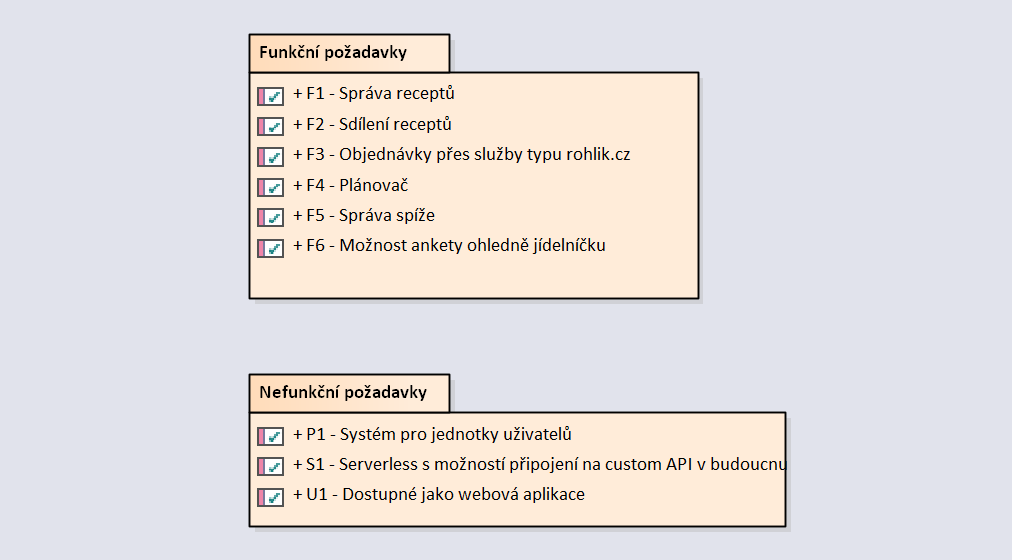
\includegraphics[width=\textwidth]{images/pozadavky}
    \caption{Model požadavků} \label{picture:recipeo:pozadavky}
\end{figure}

\section{Existující řešení}

\subsection{Webové stránky}

Porovnal jsem nejpoužívanější české portály s recepty. Některé z nich nabízejí další obsah jako například blog či magazín.

\subsubsection{Vareni.cz}

Na vareni.cz~\cite{VareniCZ} se nachází několik reklam, které jsou velké a rušivé. Není zde možné si přidat soukromý recept a sdílet ho
pouze s vybranými uživateli. Celkový koncept přidání receptu je pouze veřejný, není tedy možné si zde vytvořit sbírku
oblíbených receptů z různých portálů. Vyhledávání je možné podle názvu, ingrediencí či různých parametrů jako je druh jídla
nebo národní kuchyně. Recepty mají hodnocení od jedné do pěti hvězdiček.

Na stránce konkrétního receptu je shrnutí nejdůležitějších vlastností, tedy název, krátký popis, hodnocení a čas vaření.
Také v hlavičce kolují různé komentáře. Výhodou jsou návrhy podobných receptů. Naopak velmi špatné je rozložení seznamu ingrediencí
a postupu přípravy. Tato část je velmi nepřehledná a je nerozeznatelné kde recept končí a začínají jiné recepty.

Jsou zde kuchařky, ale než že by byly tématické nebo měli společného autora, přišlo mi, že se jedná se o náhodnou kolekci receptů,
kde je jich často více než tisíc.

Celkem hezký nápad jsou fotorecepty. Uživatele provedou celým vařením pomocí kroků, přičemž u každého je fotodokumentace jak daný krok
provést.

\begin{figure}[H]
    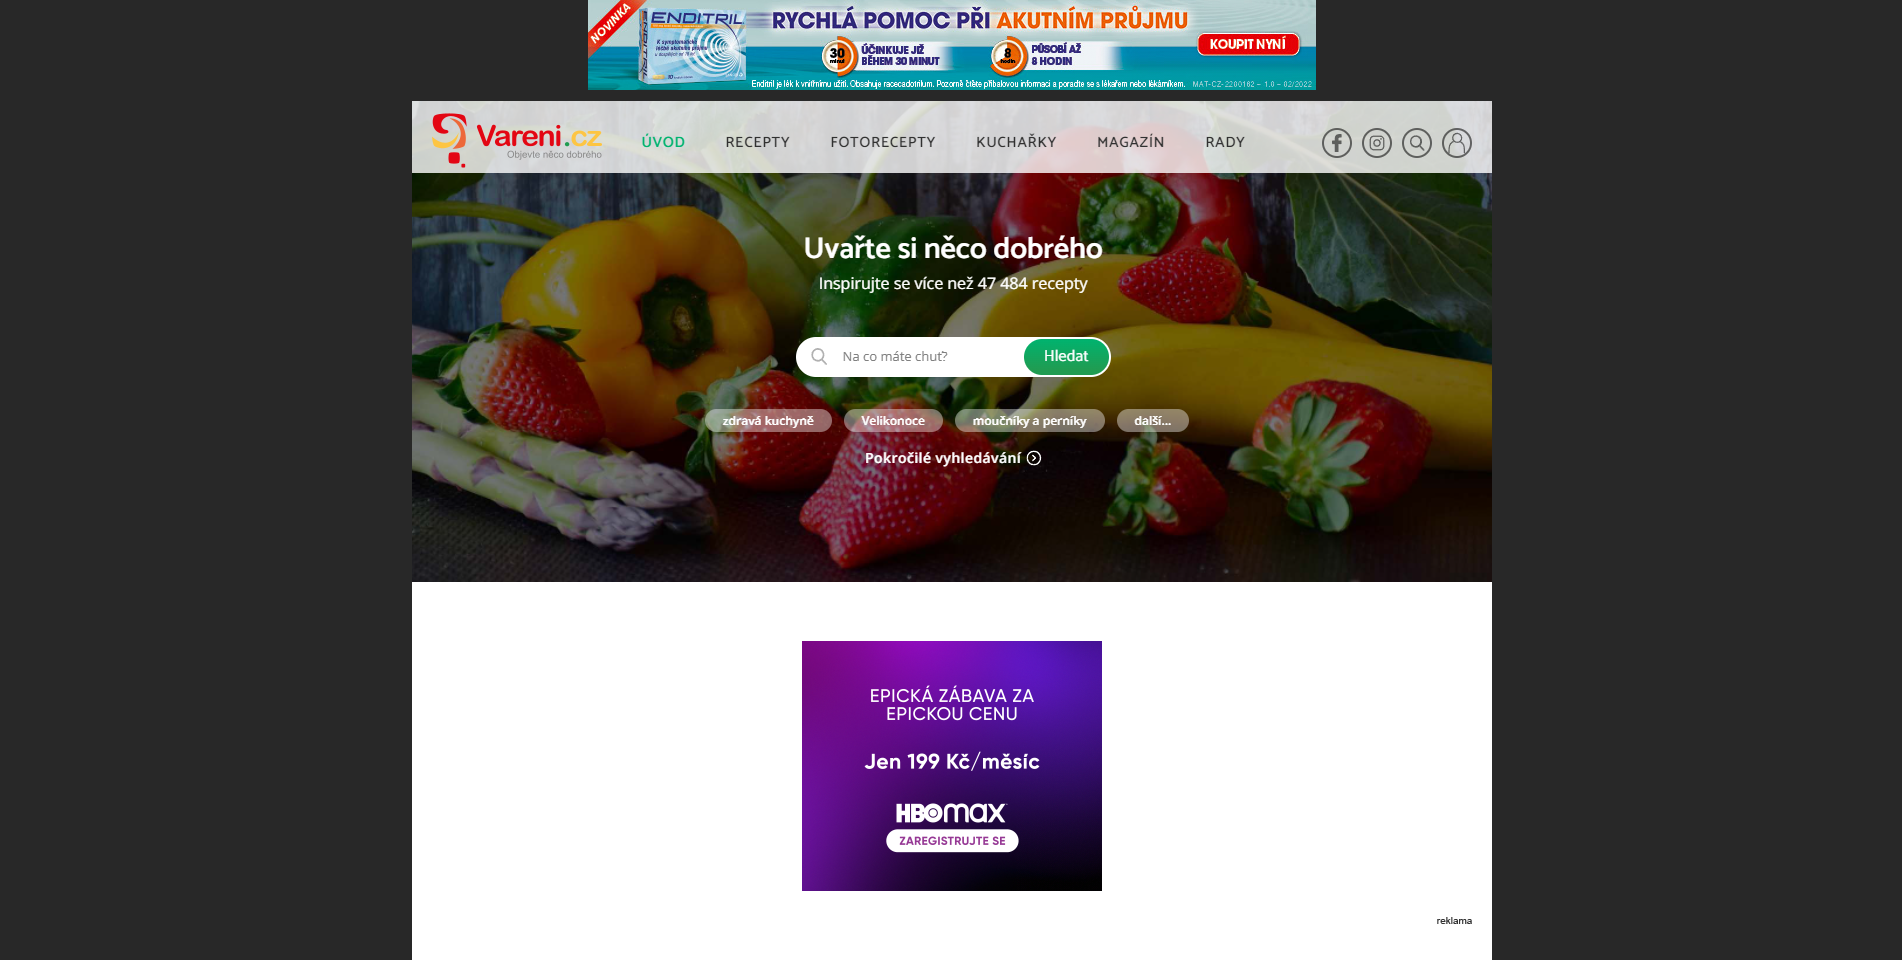
\includegraphics[width=\textwidth]{images/varenicz-uvodni-stranka}
    \caption{Hlavní stránka vareni.cz} \label{picture:varenicz:uvodni-stranka}
\end{figure}

\subsubsection{Toprecepty.cz}

Na tomto portálu~\cite{TopreceptyCZ} byla bohužel nefunkční registrace, takže jsem nemohl nahlédnout na funkce poskytované přihlášeným
uživatelům. Opět zde byla přítomna velká reklama, která zabírala většinu stránky. Jinak byl web navrhnut přehledně,
ale narazil jsem na několik nefunkčních prvků na mobilním zobrazení. Zhodnotit přidání receptů a jak funguje jejich
sdílení zhodnotit nemohu, kvůli výše zmíněným problémům. Našel jsem funkci podobnou doporučování receptů, avšak se
pravděpodobně jedná o náhodné doporučení, které nemá nic společného s tím co má uživatel rád. Dále je na webu dostupný
online magazín, kde jsou různé články týkající se gastronomie.

\begin{figure}[H]
    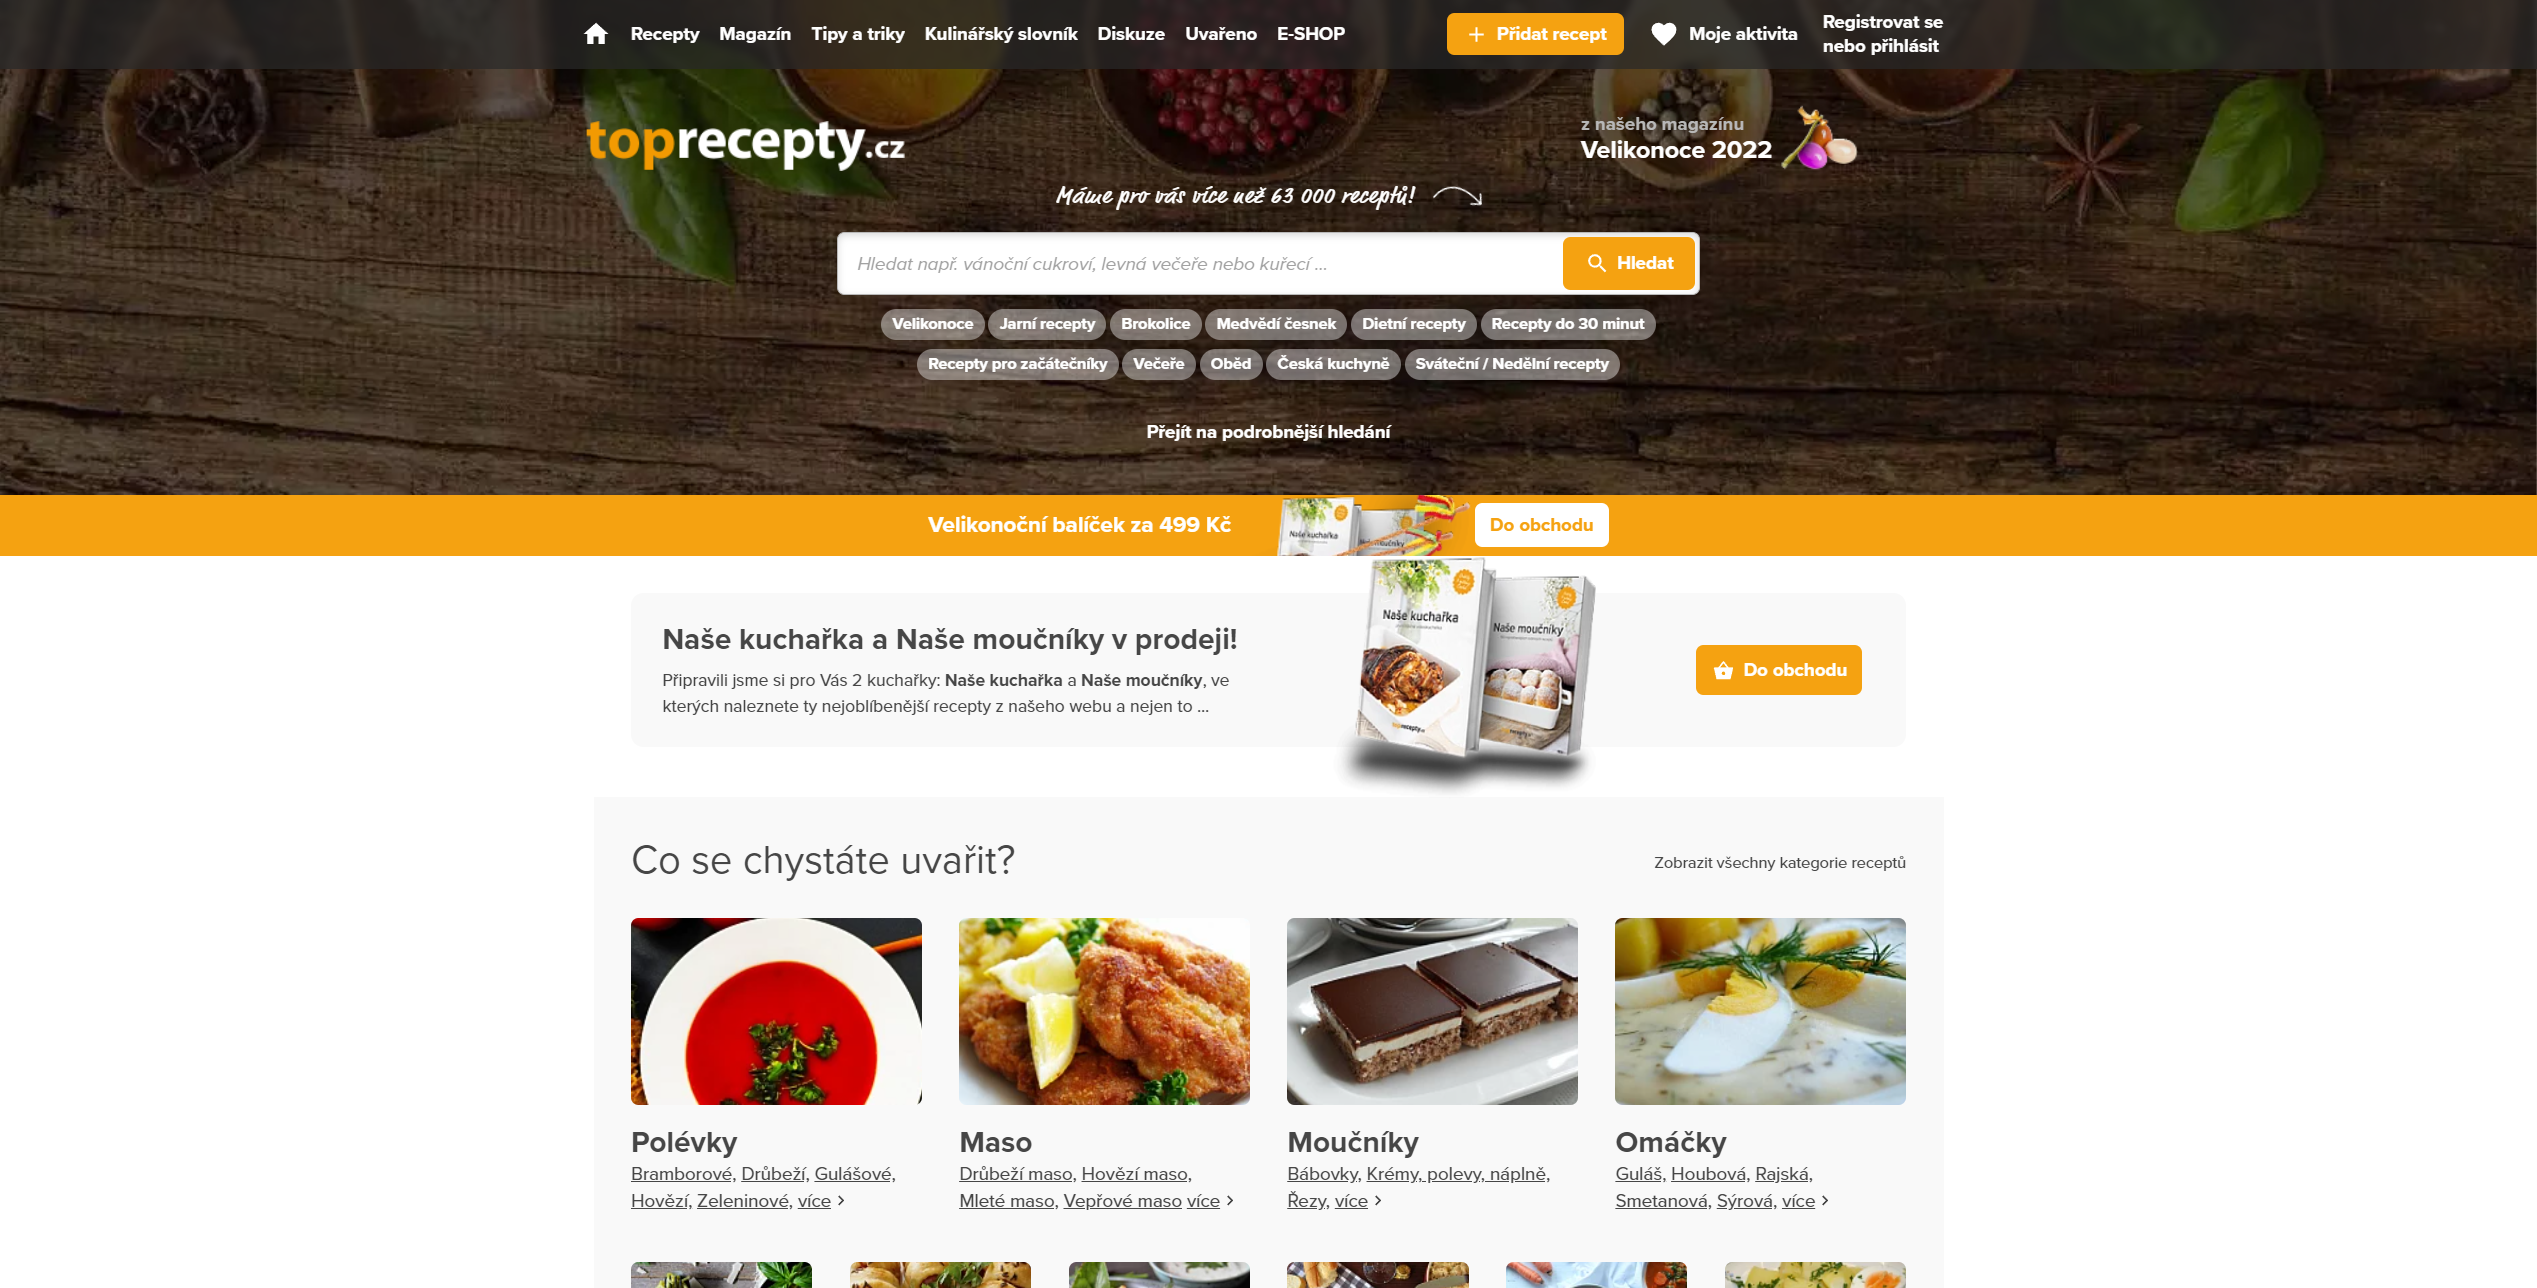
\includegraphics[width=\textwidth]{images/topreceptycz-uvodni-stranka}
    \caption{Hlavní stránka toprecepty.cz} \label{picture:topreceptycz:uvodni-stranka}
\end{figure}

\subsubsection{Recepty.cz}

I třetí zástupce~\cite{ReceptyCZ} existujících řešení používá reklamu přes celou stránku okolo jejího obsahu. Podobně jako toprecepty.cz
je zde magazín obsahující příspěvky na spoustu témat o vaření. U přidání receptu nebylo napsané, co se s receptem stane,
zda bude veřejný nebo se zobrazí pouze mě. Po kliknutí na tlačítko \uv{Uložit recept}, se zobrazila stránka s nadpisem
\uv{Recept čeká na schválení}. Nebylo tedy opět možné soukromé použití.

Zobrazení receptu je podobné tomu na vareni.cz, ale přijde mi více přehledné. U kroků se zobrazují rady, které ale
nemají s daným krokem nic společného, spíše odkazují na náhodné články či recepty.

\begin{figure}[H]
    \includegraphics[width=\textwidth]{images/receptycz-uvodni-stranka}
    \caption{Hlavní stránka recepty.cz} \label{picture:receptycz:uvodni-stranka}
\end{figure}

\subsection{Mobilní aplikace}

Vzhledem k tomu, že se kromě zobrazení na počítači snažím vytvořit i aplikaci přizpůsobenou pro mobilní zařízení, není od věci
si projít aplikace obsahující recepty. Vlastním telefon s operačním systémem Android a tak jsem stahoval aplikace z Obchodu Play.
Přístup k iOS nemám a tak jsem aplikace pro tento OS nezkoumal.

\subsubsection{Vareni.cz}
Tato aplikace~\cite{VareniCZAplikace} je založena na webové stránce, kterou jsem již popsal dříve. Recepty jsou v nabídce stejné, což by se dalo očekávat,
když jde o stejného tvůrce, ale co mě překvapilo je, že v aplikaci je pouze omezené množství receptů a více jich nelze získat, pouze
po připojení přes webový prohlížeč. Aplikace má jednu obrovskou výhodu a to sice že nezobrazuje žádné reklamy nebo se mi alespoň na
žádnou nepodařilo narazit.

Po spuštění se uživateli zobrazí základní rozdělení receptů do kategorií jako polévky, přílohy nebo hlavní chody. Je to jediná možnost
jak filtrovat recepty a jinak lze vyhledávat podle slovního spojení, ale to se mi moc neosvědčilo, protože výsledky neodpovídaly slovům,
která jsem zadal. Dále si uživatel může označit oblíbené recepty, které se mu zobrazí pod speciální záložkou.

Aplikace je celkově velmi chudá a nabízí omezené množství funkcí narozdíl od webové verze.

\subsubsection{Jíme zdravě}
Jako další aplikaci jsem si vybral Jíme zdravě~\cite{JimeZdrave}. Aplikace měla výborné hodnocení a poměrně vysoký počet stažení na to o jakou aplikaci se jedná.
Po spuštění se musí uživatel přihlásit přes Facebook nebo pomocí emailu. Poté už se zobrazí hlavní obrazovka aplikace, tedy záložka \uv{Objevuj}.
Aplikace má líbivý a moderní vzhled a dá se v ní lehce orientovat. Zobrazení receptu je organizované a přehledné. Je možné si zakoupit
prémium verzi a tím uživatel dostane přístup ke všem receptům a kuchařkám, které aplikace obsahuje.

\begin{table}[H]\centering
\caption{~Porovnání základní a premium verze}\label{tab:jimezdrave:zakladpremium}
\begin{tabular}{l|c|c}
    Typ		                                    & Základ    & Premium   \tabularnewline \hline
    Ukládání receptů		                    & Ano		& Ano       \tabularnewline \hline
    Poznámky k receptům	                        & Ano       & Ano       \tabularnewline \hline
    Hodnocení receptů	                        & Ano		& Ano       \tabularnewline \hline
    1000 receptů z kuchařek	                    & Ne		& Ano       \tabularnewline \hline
    Přístup k videokurzům	                    & Ne		& Ano       \tabularnewline \hline
    Vaření z lednice / spíže                    & Ne        & Ano       \tabularnewline \hline
    Recepty dostupné offline                    & Ne        & Ano       \tabularnewline \hline
    Appka bez reklam                            & Ne        & Ano       \tabularnewline \hline
    Nákupní seznam                              & Ne        & Dostupné v květnu 2022    \tabularnewline \hline
    Týdenní plánovač jídel                      & Ne        & Dostupné v červnu 2022    \tabularnewline \hline
    Vybrané recepty na míru                     & Ne        & Dostupné v červenci 2022  \tabularnewline
\end{tabular}
\end{table}

Zdá se tedy, že Jíme zdravě je nejblíže k aplikaci, kterou se snažím vytvořit já, ale zaměřuje se výhradně na zdravé recepty.

\subsection{Závěr}

Existující řešení na vyhledávání receptů nabízejí pouze veřejné recepty a mají spoustu reklam. Moje řešení bude poskytovat
možnost soukromé sbírky receptů a jejich sdílení s vybranými uživateli či pomocí odkazu.

Sestavil jsem tabulku s hodnocením od jedné do pěti, stejné jako se používá ve škole\footnote{Hodnocení recipeo.cz je na základě návrhu, ne podle výsledné verze.}.
Každý aspekt jsem ohodnotil pro všechny stránky, které jsem zahrnul v porovnání a přidal jsem skóre, které je v souladu s parametry mojí aplikace.

\begin{table}[H]\centering
    \caption{~Porovnání konkurenčních řešení}\label{tab:recipeo:konkurencni-reseni}
    \begin{tabular}{l|c|c|c|c}
        Typ		                & vareni.cz & toprecepty.cz & recepty.cz & recipeo.cz \tabularnewline \hline
        Reklamy		            & 4		    & 2	            & 3          & 1          \tabularnewline \hline
        Zobrazení receptu	    & 3		    & 2	            & 3          & 1          \tabularnewline \hline
        Doporučování receptů	& 2		    & 2	            & 2          & 3          \tabularnewline \hline
        Model sdílení	        & 4		    & 4	            & 4          & 2          \tabularnewline \hline
        Zjednodušení nákupu	    & 4		    & 3	            & 2          & 1          \tabularnewline
    \end{tabular}
\end{table}

\section{Nákup surovin}

Vedoucí práce již dříve používal aplikaci Zdravý stůl~\cite{ZdravyStul}. Tam bylo možné si jídlo objednat přes rohlik.cz (vložit do košíku).
Tudíž jsme chtěli tuto funkcionalitu zachovat a přidat možnosti jako například vytvoření objednávky u konkurence - kosik.cz
či zobrazení interaktivního nákupního listu.

\subsection{Komunikace s Rohlíkem a Košíkem}

\subsubsection{Rohlík}
Nejdříve jsem se rozhodl kontaktovat Rohlík. Po pár vyměněných e-mailech jsem obdržel celou dokumentaci k jejich API,
které nám otevřelo spoutu možností i do budoucna. Například bych mohl sledovat, jaké suroviny jsou právě ve slevě a
podle toho doporučovat jídla. Toto API je primárně používané přímo Rohlíkem pro jejich mobilní aplikaci. Avšak jsem se
dozvěděl, že mají již ve vývoji rozhraní určené přímo pro partnery, ale zatím nevědí, kdy bude dostupné.

\subsubsection{Košík}
Od Košíku jsme dostali pozvání na schůzku, kde jsme si mohli prohlédnout i jejich kanceláře. Na schůzce jsme hned na začátku
zjistili, že žádné API narozdíl od Rohlíku ještě dostupné není, ale už na něm pracují. Plánované období vydání je
první kvartál roku 2022. Pro jeho využití je však potřeba OAuth server, který zatím není dostupný.

Jako alternativu jsme dohromady vymysleli link na přidání surovin přímo do košíku, ze kterého nakonec sešlo, protože jsme
poté objevili funkci \uv{Nákupní lístek}, kterou bychom mohli využít. Odeslali bychom seznam surovin a uživatel by si je poté
mohl vybrat přímo z nabídky na Košíku. Nakonec jsme zjistili, že by se Košíku hodilo rozrůst sbírku receptů a bylo by možné
pro uživatele naší aplikace nabínout jejich recepty Košíku, který by je následně odkoupil. % TODO: Obrázek

\subsubsection{Závěr}
Moje hlavní zaměření v této práci je na \emph{frontend}. Tudíž jsem se zaměřil na pohodlí, design a použitelnost pro uživatele
a rozšířené funkce jsem pouze zanalyzoval. Na \emph{backendu} jsem se zaměřil pouze na funkční strukturu dat a jeho rozšiřitelnost
v budoucnu, až bude potřeba tyto funkce, jako je například objednávání surovin, implementovat.

